\documentclass[a4paper,10pt]{article}

\usepackage[latin1]{inputenc}
\usepackage{amsfonts}
\usepackage{amsmath}
\usepackage{amssymb}
\usepackage{amsthm}
\usepackage[T1]{fontenc}
\usepackage[dvips]{graphicx}

\author{Kefei Lu}
\title{The Blahut Algorithm For Estimating Channel Capacity}
\date{2008-05-05}

\begin{document}

\maketitle

%\begin{abstract}
%The report mainly illustrate how the Blahut algorithm for estimating channel capacity is implemented. 
%\end{abstract}

\section{Introduction}
% Here we illustrate the algorithm. Give flow charts. etc.
Blahut Algorithm is an iterative way to estimate the channel capacity and rate-distortion functions in information theory. 

In this project, the Blahut algorithm for estimating capacity-expense function is implemented using C programming language. The algorithm is implemented in an object-oriented fashion and is easy to use. The vector and matrix manipulation is based on the GNU Scientific Library. The algorithm is provided as a programming library so that it can be easily integrated in any other applications.

Figure \ref{fig:unconstrained_cap},\ref{fig:constrained_cap} show the algorithm for estimating the unconstrained capacity and the constrained capacity. They were originally published in R.E.Blahut's paper \textit{Computation of Channel Capacity and Rate-Distortion Functions} in 1972. 

\begin{figure}
 \centering
 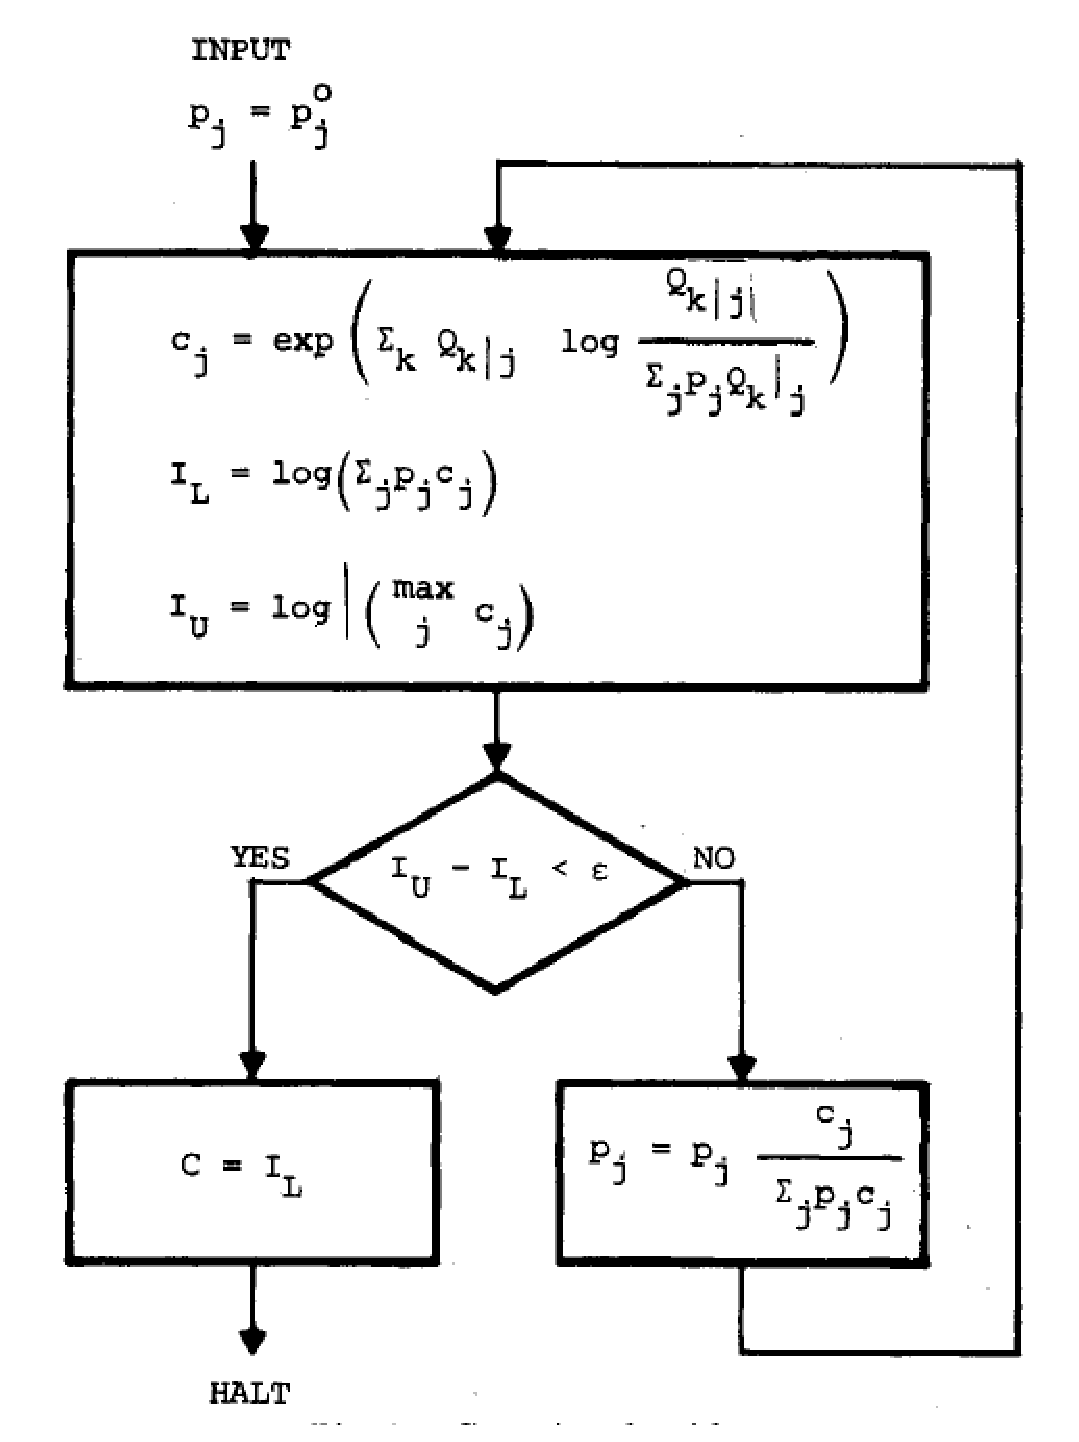
\includegraphics[width=0.5\textwidth]{pic/unconstrained_cap.eps}
 % unconstrained_cap.eps: 1179666x1179666 pixel, 300dpi, 9987.84x9987.84 cm, bb=14 14 516 690
 \caption{Flow chart illustration for computing unconstrained channel capacity}
 \label{fig:unconstrained_cap}
\end{figure}
\begin{figure}
 \centering
 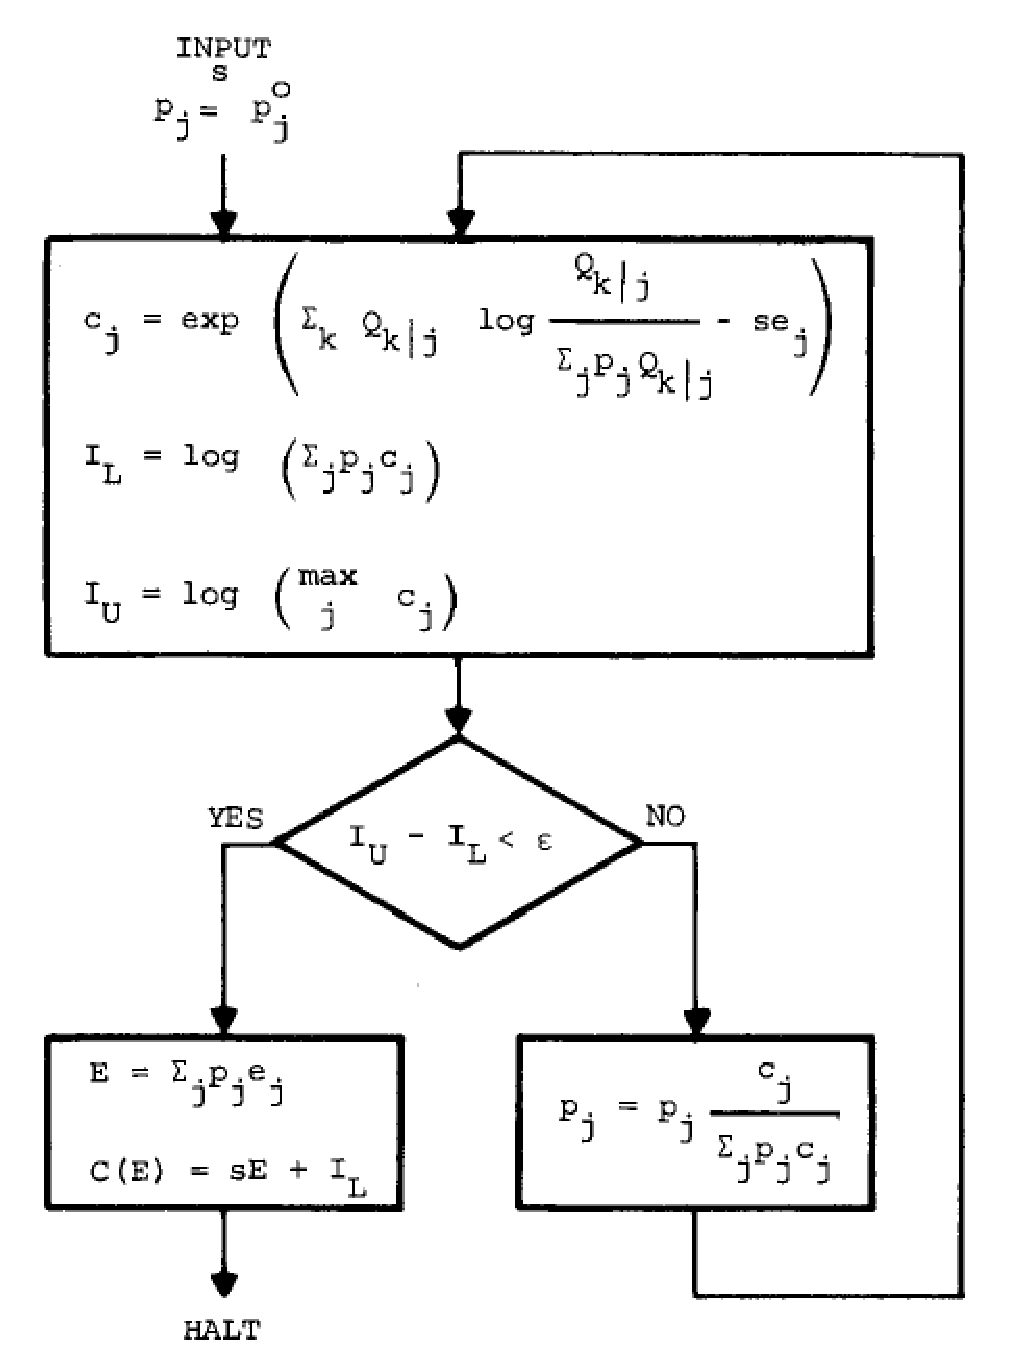
\includegraphics[width=0.5\textwidth]{pic/constrained_cap.eps}
 % unconstrained_cap.eps: 1179666x1179666 pixel, 300dpi, 9987.84x9987.84 cm, bb=14 14 516 690
 \caption{Flow chart illustration for computing constrained channel capacity}
 \label{fig:constrained_cap}
\end{figure}

\section{Case Studies}
% Describe the problem. Analize theoretically first, then show algorithm results.
\subsection{Binary Symmetric Channel}
The forward transition matrix of a binary symmetric channel can be expressed as:
\[\mathbf{Q} = \left[
\begin{array}{ccc}
1-p & p \\
p & 1-p \\
\end{array}
\right],\]
where $p$ is the cross over probability.

The unconstrained capacity is defined as:
\begin{equation}
 C = \max_{\mathbf{p}}{I(X,Y)}
\end{equation}
and is maximized to:
\begin{equation}
 C = 1 - \mathcal{H}(p), 
\end{equation}
when the input distribution is uniform distribution: $p^* = [0.5,0.5]^T$. 

For a special case when the cross-over probability $p=0$, i.e., all bits are transmitted reliably, $C = 1-\mathcal{H}(0) = 1\ bits/c.c$.

Given an expense schedule $\mathbf{e}$, and a constraint on the average expense of input $\sum_{x}{p(x)e(x)}\leq E$, the constrained capacity can be defined as:
\begin{equation}
 C(E) = \max_{\mathbf{p}\in P_E} {I(X;Y)} = \max_{\mathbf{p}\in P_E} {I(\mathbf{p};\mathbf{Q})},
\end{equation}
where $P_E$ is the constrained set and is defined as:
\begin{equation}
 P_E = \left\lbrace \mathbf{p}: p(x)\geq 0, \sum_{x}{p(x)}=1, \overline{E}=\sum_{x}{p(x)e(x)} \leq E \right\rbrace 
\end{equation}
If the expense schedule is set to $e=[0\ 1]^T$ for the BSC, we have $E_{min}=0$ when $\mathbf{p}=[1,\ 0]^T$, i.e., only $X=0$ is transmitted to avoid any expense on transmission. Thus we expect that the corresponding channel capacity $C_{min}=0$ because no information is conveyed in the transmission. Likewise, $C_{max}=1-\mathcal{H}(p)\ bits/channel\ use$ is achieved when $p^*_{\ E_{max}}=p^*=[0.5\ 0.5]^T$. And $E_{max}=0.5$.

For any $E\in[E_{min},\ E_{max}]$, since $p^*=[1-\alpha,\ \alpha]^T$, we have $\alpha=E$, therefore $p^*=[1-E,\ E]^T$. And the corresponding channel capacity can be expressed as
\begin{equation}
 C=I(\mathbf{p};\mathbf{Q})=\sum_{x}{p_x {\sum_{y} {p_{y|x}\log{\frac{p_{y|x}}{p_y}}}}}\ .
\end{equation}

Figure \ref{fig:bsc_cap} shows the result obtained by running the Blahut algorithm in the binary symmetric channel case, and $e=[0,\ 1]^T$. Different cross-over probabilities are tried and plotted on the same figure.
\begin{figure}
 \centering
 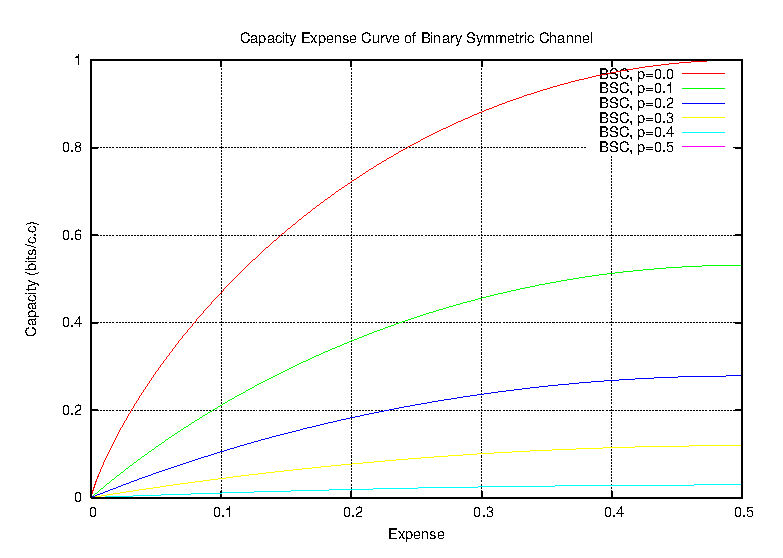
\includegraphics[bb=50 50 410 302]{pic/bsc_cap.eps}
 % bsc_cap.eps: 1179666x1179666 pixel, 300dpi, 9987.84x9987.84 cm, bb=50 50 410 302
 \caption{Capacity Expense Curve of Binrary Symmetric Channel for different cross-over probabilities. $e=[0\ 1]^T$}
 \label{fig:bsc_cap}
\end{figure}

\subsection{Example 1}
The forward transition matrix looks like the following:
\[
 \mathbf{Q} = \left[ 
\begin{array}{cccc}
1 & 0 & 0 & 0 \\ 
0 & q & 1-q & 0 \\ 
0 & 0 & 0 & 1
\end{array}\right] 
\]

As can be observed, $H(X|Y)=0$, i.e., when output is observed, the input can be uniquely determined. This is because that channel can be viewed as three parallel reliable subchannels. As can be expected, changing on parameter $q$ has no effect on the overall channel capacity.

The unconstrained capacity can be calculated as the following:
\begin{equation}
 C=\max_{\mathbf{p}} {I(X;Y)}=\max_{\mathbf{p}} {H(X)-H(X|Y)},
\label{eq:ex1_C}
\end{equation}
since $H(X|Y)=0$, eq. \ref{eq:ex1_C} can be further written as:
\begin{equation}
 C=\max_{\mathbf{p}}{H(X)},
\end{equation}
$H(X)$ is maximized when $\mathbf{p}=[1/3\ 1/3\ 1/3]^T$. And $C=\log_2{3}\approx1.59\ bits/channel\ use$.

When $e=[0,1,0]^T$ is assigned as expense schedule, $E_{min}$ is achived when $p=[\alpha/2\ 0\ \alpha/2]^T$, because of channel symetry. $C_{min}=log_2{3}\ bits/channel\ use$ as the channel reduces to BSC in this case.

Naturally, $C_{max}=C_{unconstrained}$ is achieved as $\mathbf{p}=[1/3\ 1/3\ 1/3]^T$. Therefore $E_{max}=1/3$ in this case.

Figure \ref{fig:example1_cap} shows the Blahut algorithm estimation on this channel for expense schedule $e=[0,1,0]^T$.
\begin{figure}
 \centering
 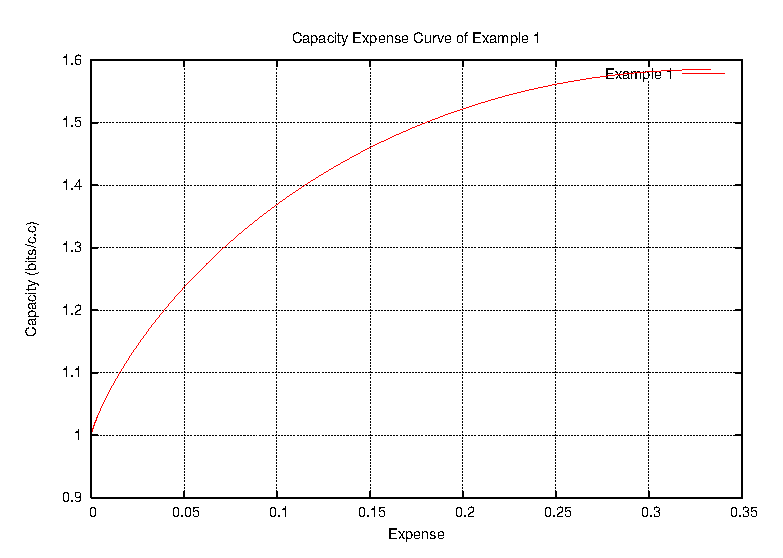
\includegraphics[bb=50 50 410 302]{pic/example1_cap.eps}
 % example1_cap.eps: 1179666x1179666 pixel, 300dpi, 9987.84x9987.84 cm, bb=50 50 410 302
 \caption{Capacity Expense Curve of Channel Described in Example 1. $e=[0,1,0]^T$.}
 \label{fig:example1_cap}
\end{figure}
As shown in the figure, the estimation agrees with theoretical analyse perfectly.

\subsection{Example 2}
The forward transition matrix looks like:
\begin{displaymath}
% use packages: array
\mathbf{Q}=\left[ 
\begin{array}[c]{ccc}
1-p & p & 0 \\ 
0 & 1 & 0 \\ 
0 & p & 1-p
\end{array}\right], 
\end{displaymath}
with expense schedule $e=[1,0,1]^T$.

It's easy to show from Kuhn-Tuckor condition that the unconstrained capacity can be achieved when $p^*=[\frac{1-\alpha}{2}\ \alpha \frac{1-\alpha}{2}]^T$. The unconstrained capacity is
\begin{equation}
 C=log{\frac{1/p}{1+\alpha^*\left(\frac{1-p}{p}\right)}}
\end{equation}

For example, $p=1/3$, we solve for
\begin{equation}
 \frac{1-\alpha}{1+2\alpha}=2\left(\frac{1}{3}\right)^{3/2}
\end{equation}
in which case
\[\alpha^*=\frac{3\sqrt{3}-2}{3\sqrt{3}+4}\approx0.348\],
and 
\[C=log{\frac{3}{1+2\alpha^*}}\approx0.824\ bits/channel\ use\].

Now let's consider capacity expense function C(E). Clearly we have $E_{min}=0$ which is achieved when $p_{E_{min}}^*=[0,1,0]^T$. The corresponding capacity is $C(E_{min})=0$.

For $E\geq0$, $p_E^*=[\frac{1-\alpha_E^*}{2},\alpha_E^*,\frac{1-\alpha_E^*}{2}]^T$, due to channel symmetry. Since $1-\alpha_E^*=E$, we have
\begin{equation}
 p_E^*=[E/2,1-E,E/2]^T
\end{equation}
Finally we have
\begin{equation}
 C(E)=I(p_E^*;Q)=H(Y)-H(Y|X)=E(1-p)+\mathcal{H}(E(1-p))-E\mathcal{H}(p)
\end{equation}
For different value of $p$, we have different $C(E_{max})$ and the corresponding $E_{max}$. For the example that $p=1/3$, we have $C(E_{max})\approx0.824$, when $E_{max}=1-\alpha^*\approx0.652$. 

The case when $p=1/3$ is estimated using Blahut algorithm and is shown in figure \ref{fig:example2_p0.3}. Also, cases with different $p$ values are plotted together in figure \ref{fig:example2_cap}.

\begin{figure}
 \centering
 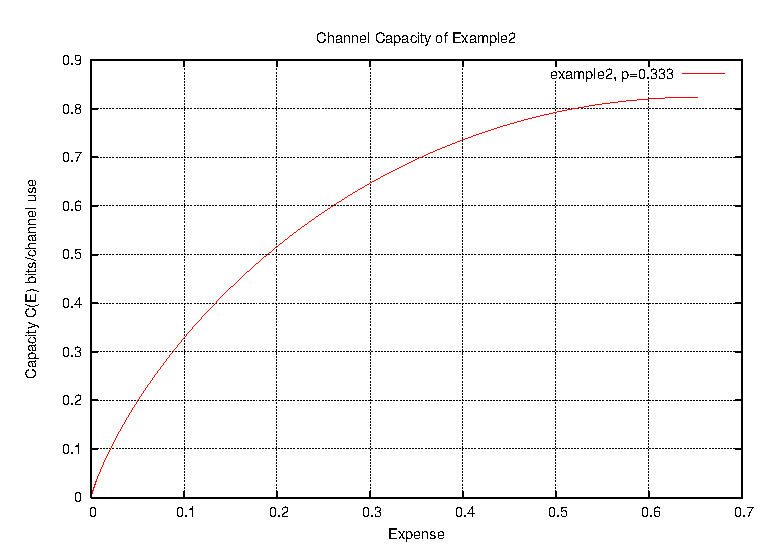
\includegraphics{pic/example2_cap_p0.3.eps}
 % example2_cap_p0.3.eps: 360x252 pixel, 72dpi, 12.70x8.89 cm, bb=0 0 360 252
 \caption{Capacity Expense Curve of Example 2 with p=1/3}
 \label{fig:example2_p0.3}
\end{figure}

\begin{figure}
 \centering
 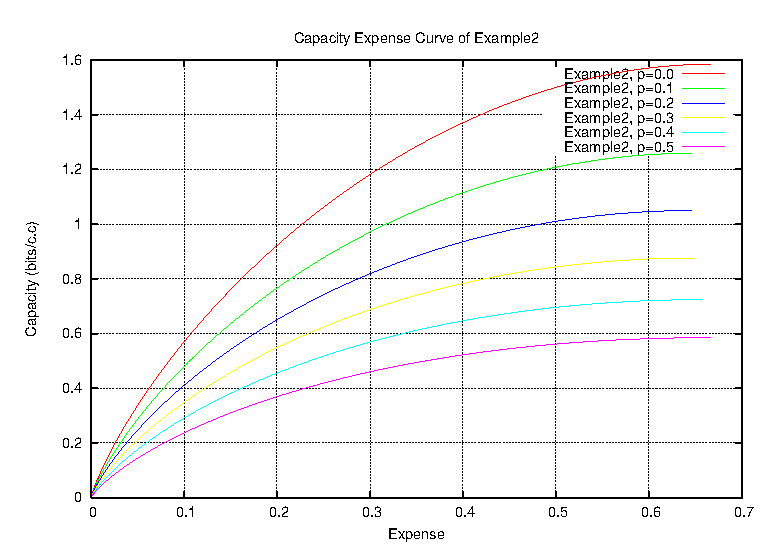
\includegraphics[bb=50 50 410 302]{pic/example2_cap.eps}
 % example2_cap.eps: 1179666x1179666 pixel, 300dpi, 9987.84x9987.84 cm, bb=50 50 410 302
 \caption{Capacity Expense Curve of Example 3 with different values of p}
 \label{fig:example2_cap}
\end{figure}

\section{Library Usage}
% Manual for the library.
\subsection{Installation}
To use the library, one must have GNU Scientific Library (GSL) installed. GSL is used in this library for mathematical and matrix manipulations. In fact, this library is intend to be an extension of GSL. 

Two optional software are GNU Plot and GNU Octave, which are used to plot the curves.

To build the library, copy it to the desired location, and type \verb|make| to build the shared library file ``libblahut.so''. To link with this library, one must:
\begin{enumerate}
 \item Include \verb|blahut.h| in the source files
 \item Include /path/to/lib (path where ``libblahut.so'' locates) to the \verb|LD_LIBRARY_PATH| environment
 \item At the link stage, append linking options \verb|-L/path/to/lib -lm -lblahut `gsl-config --libs`| to the linker command
\end{enumerate}

\subsection{Objects and Meathods}
\subsection{Utilities}
 
\end{document}
